\begingroup
\setlength{\tabcolsep}{15pt} % Default value: 6pt
\begin{figure}[!htb]
    \centering
    \begin{tabular}{cccc}
        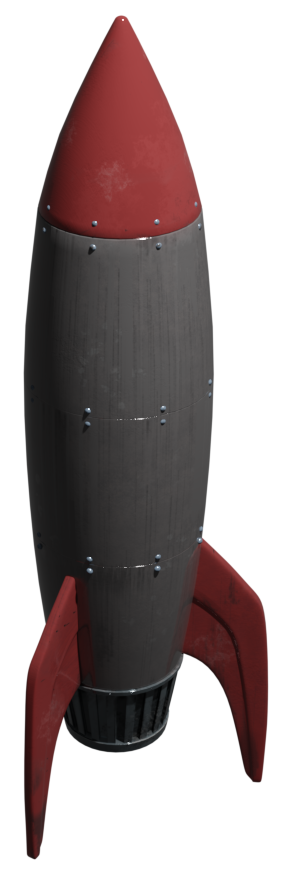
\includegraphics[width=0.1\textwidth]{figures/rocket.png}
        & 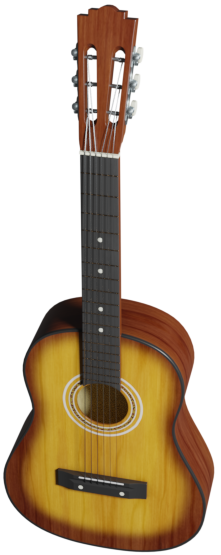
\includegraphics[width=0.13\textwidth]{figures/guitar.png}
        & 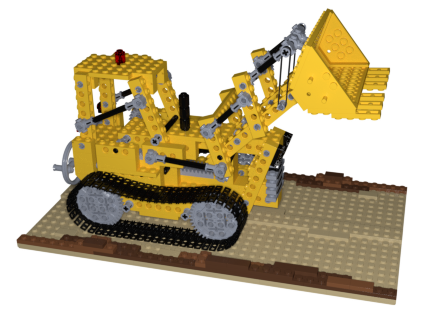
\includegraphics[width=0.30\textwidth]{figures/lego.png}
        & 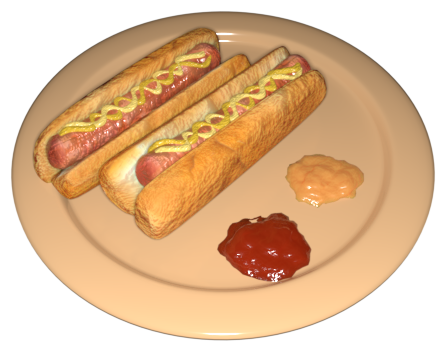
\includegraphics[width=0.25\textwidth]{figures/hotdog.png} \\
        (a) Rocket & (b) Guitar & (c) Lego & (d) Hotdog
    \end{tabular}
    \caption{
    Preview samples of the created datasets.
    All the datasets are created from the very beginning.
    (a) \cite{boucher2019rocket} and (b) \cite{legalov2020guitar} are created from publicly available 3D models in Blender \cite{blender}.
    (c) and (d) are created from 3D models that are publicly available withing NeRF work \cite{mildenhall2019local}.
}
\label{fig:dataset_preview}
\end{figure}
\endgroup